\chapter{Methods in ...}

% \section{Voxelnet}
% VoxelNet is an End-to-End Learning for Point Cloud Based 3D Object Detection. The work is described in Yin Zhou and Oncel Tuzel's paper: \cite{https://doi.org/10.48550/arxiv.1711.06396}.

% In order to implement this work, the following git repo is adapted: \url{https://github.com/qianguih/voxelnet}. This repo contains a pre-trained model, trained to detect cars from the velodyne lidar data provided by the KITTI dataset.

% \section{ViperX 300 Robot Arm}
% In order to operate the Trossen Robotics ViperX 300 Robotic Arm, Their ROS 2 packages are utilised.
% These can be found here: \url{https://docs.trossenrobotics.com/interbotix_xsarms_docs/}.




\section{Hardware Configuration}
Figure \ref{fig:example_drawio} is an example of drawio figure.

\begin{figure}[H]
  \centering
  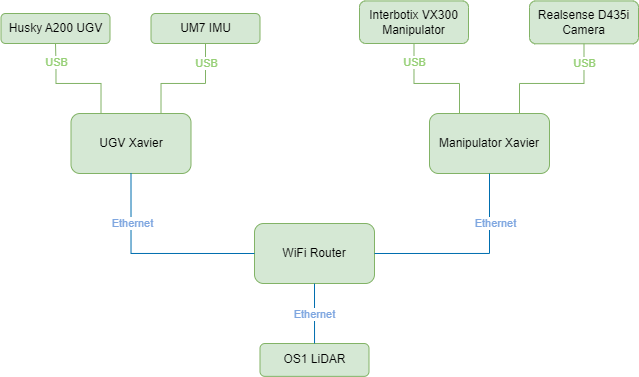
\includegraphics[width = 0.6\textwidth]{Figures/example_figure.drawio.png}
  \caption{Example of drawio figure}
  \label{fig:example_drawio}
\end{figure}
